\documentclass{amia}
\usepackage{graphicx}
\usepackage[labelfont=bf]{caption}
\usepackage[superscript,nomove]{cite}
\usepackage{color}
\usepackage{graphicx}

\begin{document}

\title{Tailoring Clinical Performance Feedback Using Semantic Technology}
\author{Zach Landis-Lewis, PhD, MLIS$^{1}$, Colin A. Gross$^{1}$, Cooper Stansbury$^{2}$, Dahee Lee$^{1}$, Veena Panicker$^{1}$}
\institutes{
    $^1$University of Michigan, Ann Arbor, MI\\
}

\maketitle

\section*{Background}

Clinical quality dashboards and reports, though ubiquitous in healthcare organizations, are often not useful for improving practice\cite{ivers2012, tuti2017}. Cognitive theories describe two ways in which visual information displays in dashboards and reports can influence clinical practice (i.e. behavior). Firstly, theories describe the cognitive processing of displays for a task (e.g. comparison, trend analysis) and a domain problem (e.g. maintain awareness of my performance relative to peers)\cite{zhang1996, munzner2014}. Secondly, cognitive theories introduce causal pathways through which performance displays can influence practice via mechanisms such as changing motivation and awareness\cite{kluger1996}. These casual pathways commonly depend on situational factors that can change over time, such as the presence of a performance gap between a healthcare professional and a peer-based benchmark. Based on these pathways, the optimal visualization of performance for an individual may differ at any given reporting interval, creating a need to tailor reports for a recipient's situation. 

Knowledge-based systems (KBSs) use explicit representations of knowledge to reason about a set of facts in a domain\cite{neapolitan2018}. A KBS approach to clinical quality reporting could 1) use causal pathways to situationally tailor reports, and 2) to generate data about causal pathway effectiveness for learning to improve report tailoring. The objective of this research is to develop and evaluate a KBS for clinical quality reporting, applied to the clinical domain of obstetric care quality.


\section*{Performance Feedback Tailoring System}

\begin{figure}[h!]
\centering
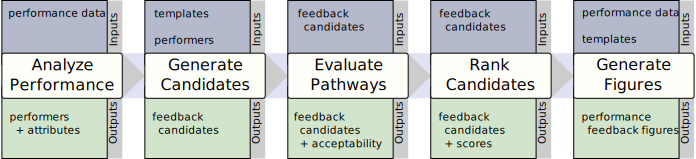
\includegraphics[scale=.65]{figures/overview_abbreviated.png}
\caption{Feedback Tailoring Overview.}
\label{fig1}
\end{figure}

We designed the system as a suite of modular applications that form a software pipeline (Figure 1). The applications in the pipeline depends on the prior development of 3 components: 1) a user-centered report template design and annotation process to develop a report template library, 2) a contextual inquiry process to develop a specification of key characteristics of the setting and recipients of the feedback reports, and 3) a knowledgebase of causal pathways through which performance feedback can influence clinical practice.
These components provide the configuration that corresponds to the specific professional environment for which the software will tailor feedback.

The pipeline begins with processing of the performance data to make inferences about the attributes of each performer (e.g. a feedback recipient). Annotation functions, written to implement the environment-specific interpretations of attributes, infer attributes of performers from the data. For example, a `performance gap' attribute could be inferred as present when performance is 5 percent or more below average; an `upward trend' is inferred as present when performance values increase by at least .5 over three consecutive time points.
Outputs of the annotation functions are collated into a set of performers with performance-data derived attributes.

Feedback candidates are intermediate constructs generated from attributes of performers and figure templates.
Concatenating the attributes from a performer and a template to produce a feedback candidate provides a computational and conceptual convenience.
It assembles all the attributes that a psychological theory will operate on in a single container.
Template attributes, unlike performer attributes, are known before runtime.
For instance, a template that can display performance from multiple performers would have a peer comparison attribute as will all the candidates generated from this template.
Combining each recipient in turn with each template yields the cartesian product of the sets.

Causal pathways describe relationships between the attributes of a recipient and feedback figure.
They are modeled from theories of performance feedback interventions\cite{kluger1996}, and are applied to indicate which candidates are acceptable.
The implementation is a set of preconditions which must be present in a candidate to assert the candidate is acceptable.
For example, one might assert that a candidate is acceptable if it displays a performance gap, the recipient has no capability barriers, and there is a negative gap in the performance.
Applying preconditions of causal pathways in this way results in the set of candidates with attributes added that indicate which causal pathways assert the candidate is acceptable.

Figures are generated by passing performance data to figure templates.
In the even that multiple candidates are indicated as acceptable, multiple figures will be generated.
Multiple figures will be generated for a performer if multiple different candidates are indicated as acceptable.
The result is a set of performance feedback figures for each performer.

Resolution of which causal pathway, and resulting figure, is the most acceptable and appropriate remains to be determined experimentally.
The figures generated for each performer can be presented to them for evaluation.
The performer receiving the feedback figures could evaluate each for acceptability and appropriateness.
The acceptability and appropriateness of each figure can be attributed back to the causal pathways that selected for generating the figure.
Sufficient replication accross many similar environments can lead to an inter-pathway scoring model that permits the selection of a single most appropriate performance feedback for individual recipients.

\section*{Preliminary results}

The initial work has created implementations of pipeline steps and two ontologies to support serializing and reasoning about the components.
Performance data processing has been implmeneted in R\cite{rcoreteam2018} as a configurable application\cite{bitstomach2018} with a command line interface.
Candidate generation has been implemented in Ruby as a command line tool\cite{cansmash2018}.
Candidate annotation by causal pathway has been implemented in R as a command line tool\cite{thinkpudding2018}.
Supporting ontologies, Causal Pathway Ontology and Feedback Intervention Display Ontology, are owl formatted ontologies conforming to the Basic Formal Ontology structure.
The later pipeline steps such as intra-theory scoring and figure generation, exist as proof of concept builds.

\makeatletter
\renewcommand{\@biblabel}[1]{\hfill #1.}
\makeatother

\bibliographystyle{unsrt}
\begin{thebibliography}{1}
\setlength\itemsep{-0.1em}

\bibitem{ivers2012}
Ivers N, Jamtvedt G, Flottorp S, Young JM, Odgaard-Jensen J, French SD, et al. Audit and feedback: effects on professional practice and healthcare outcomes. Cochrane Database Syst Rev. 2012;6:CD000259. 
\bibitem{tuti2017}
Tuti T, Nzinga J, Njoroge M, Brown B, Peek N, English M, et al. A systematic review of electronic audit and feedback: intervention effectiveness and use of behaviour change theory. Implementation Science. 2017;12:61.
\bibitem{zhang1996}
Zhang J. A representational analysis of relational information displays. International Journal of Human Computer Studies. 1996;45(1):59-74.
\bibitem{munzner2014}
Munzner T. Visualization Analysis and Design. CRC Press; 2014. 422 p. 
\bibitem{kluger1996}
Kluger AN, DeNisi A. The effects of feedback interventions on performance: A historical review, a meta-analysis, and a preliminary feedback intervention theory. Psychological Bulletin March 1996. 1996;119(2):254-84.
\bibitem{neapolitan2018}
Neapolitan RE, Jiang X. Artificial Intelligence: With an Introduction to Machine Learning, Second Edition. 2 edition. Chapman and Hall/CRC; 2018. 480 p. 

\bibitem{bitstomach2018}
Landis-Lewis Z, Gross CA. Bit Stomach: Processes performance data to assert causal pathway attributes about performers. GitHub. 2018. DOI:10.5281/zenodo.1300745.
\bibitem{cansmash2018}
Landis-Lewis Z, Gross CA. Candidate Smasher: Make performance feedback display candidates. GitHub. 2018. DOI:10.5281/zenodo.1300855.
\bibitem{thinkpudding2018}
Landis-Lewis Z, Gross CA. Think Pudding: A minimal proof of concept candidate reasoner and ontology example. GitHub. 2018. DOI:10.5281/zenodo.1300912.
\bibitem{rcoreteam2018}
R Core Team (2018). R: A language and environment for statistical computing. R Foundation for Statistical Computing, Vienna, Austria. URL https://www.R-project.org/

\end{thebibliography}


\end{document}
